% Options for packages loaded elsewhere
\PassOptionsToPackage{unicode}{hyperref}
\PassOptionsToPackage{hyphens}{url}
%
\documentclass[
  english,
  man]{apa6}
\usepackage{amsmath,amssymb}
\usepackage{lmodern}
\usepackage{ifxetex,ifluatex}
\ifnum 0\ifxetex 1\fi\ifluatex 1\fi=0 % if pdftex
  \usepackage[T1]{fontenc}
  \usepackage[utf8]{inputenc}
  \usepackage{textcomp} % provide euro and other symbols
\else % if luatex or xetex
  \usepackage{unicode-math}
  \defaultfontfeatures{Scale=MatchLowercase}
  \defaultfontfeatures[\rmfamily]{Ligatures=TeX,Scale=1}
\fi
% Use upquote if available, for straight quotes in verbatim environments
\IfFileExists{upquote.sty}{\usepackage{upquote}}{}
\IfFileExists{microtype.sty}{% use microtype if available
  \usepackage[]{microtype}
  \UseMicrotypeSet[protrusion]{basicmath} % disable protrusion for tt fonts
}{}
\makeatletter
\@ifundefined{KOMAClassName}{% if non-KOMA class
  \IfFileExists{parskip.sty}{%
    \usepackage{parskip}
  }{% else
    \setlength{\parindent}{0pt}
    \setlength{\parskip}{6pt plus 2pt minus 1pt}}
}{% if KOMA class
  \KOMAoptions{parskip=half}}
\makeatother
\usepackage{xcolor}
\IfFileExists{xurl.sty}{\usepackage{xurl}}{} % add URL line breaks if available
\IfFileExists{bookmark.sty}{\usepackage{bookmark}}{\usepackage{hyperref}}
\hypersetup{
  pdftitle={Effectiveness of distance Based suicide Intervention programs, a multi-level meta-analysis and systematic review.},
  pdfauthor={Jim Schmeckenbecher1, Katrin Rattner2, Robert J. Cramer3, Paul L. Plener4, Anna Baran5, \& Nestor D. Kapusta1},
  pdflang={en-EN},
  pdfkeywords={suicide, suicide prevention, meta-analysis, distance based intervention, remote intervention, e-based intervention},
  hidelinks,
  pdfcreator={LaTeX via pandoc}}
\urlstyle{same} % disable monospaced font for URLs
\usepackage{longtable,booktabs,array}
\usepackage{calc} % for calculating minipage widths
% Correct order of tables after \paragraph or \subparagraph
\usepackage{etoolbox}
\makeatletter
\patchcmd\longtable{\par}{\if@noskipsec\mbox{}\fi\par}{}{}
\makeatother
% Allow footnotes in longtable head/foot
\IfFileExists{footnotehyper.sty}{\usepackage{footnotehyper}}{\usepackage{footnote}}
\makesavenoteenv{longtable}
\usepackage{graphicx}
\makeatletter
\def\maxwidth{\ifdim\Gin@nat@width>\linewidth\linewidth\else\Gin@nat@width\fi}
\def\maxheight{\ifdim\Gin@nat@height>\textheight\textheight\else\Gin@nat@height\fi}
\makeatother
% Scale images if necessary, so that they will not overflow the page
% margins by default, and it is still possible to overwrite the defaults
% using explicit options in \includegraphics[width, height, ...]{}
\setkeys{Gin}{width=\maxwidth,height=\maxheight,keepaspectratio}
% Set default figure placement to htbp
\makeatletter
\def\fps@figure{htbp}
\makeatother
\setlength{\emergencystretch}{3em} % prevent overfull lines
\providecommand{\tightlist}{%
  \setlength{\itemsep}{0pt}\setlength{\parskip}{0pt}}
\setcounter{secnumdepth}{-\maxdimen} % remove section numbering
% Make \paragraph and \subparagraph free-standing
\ifx\paragraph\undefined\else
  \let\oldparagraph\paragraph
  \renewcommand{\paragraph}[1]{\oldparagraph{#1}\mbox{}}
\fi
\ifx\subparagraph\undefined\else
  \let\oldsubparagraph\subparagraph
  \renewcommand{\subparagraph}[1]{\oldsubparagraph{#1}\mbox{}}
\fi
% Manuscript styling
\usepackage{upgreek}
\captionsetup{font=singlespacing,justification=justified}

% Table formatting
\usepackage{longtable}
\usepackage{lscape}
% \usepackage[counterclockwise]{rotating}   % Landscape page setup for large tables
\usepackage{multirow}		% Table styling
\usepackage{tabularx}		% Control Column width
\usepackage[flushleft]{threeparttable}	% Allows for three part tables with a specified notes section
\usepackage{threeparttablex}            % Lets threeparttable work with longtable

% Create new environments so endfloat can handle them
% \newenvironment{ltable}
%   {\begin{landscape}\centering\begin{threeparttable}}
%   {\end{threeparttable}\end{landscape}}
\newenvironment{lltable}{\begin{landscape}\centering\begin{ThreePartTable}}{\end{ThreePartTable}\end{landscape}}

% Enables adjusting longtable caption width to table width
% Solution found at http://golatex.de/longtable-mit-caption-so-breit-wie-die-tabelle-t15767.html
\makeatletter
\newcommand\LastLTentrywidth{1em}
\newlength\longtablewidth
\setlength{\longtablewidth}{1in}
\newcommand{\getlongtablewidth}{\begingroup \ifcsname LT@\roman{LT@tables}\endcsname \global\longtablewidth=0pt \renewcommand{\LT@entry}[2]{\global\advance\longtablewidth by ##2\relax\gdef\LastLTentrywidth{##2}}\@nameuse{LT@\roman{LT@tables}} \fi \endgroup}

% \setlength{\parindent}{0.5in}
% \setlength{\parskip}{0pt plus 0pt minus 0pt}

% \usepackage{etoolbox}
\makeatletter
\patchcmd{\HyOrg@maketitle}
  {\section{\normalfont\normalsize\abstractname}}
  {\section*{\normalfont\normalsize\abstractname}}
  {}{\typeout{Failed to patch abstract.}}
\patchcmd{\HyOrg@maketitle}
  {\section{\protect\normalfont{\@title}}}
  {\section*{\protect\normalfont{\@title}}}
  {}{\typeout{Failed to patch title.}}
\makeatother
\shorttitle{Distance Based Interventions}
\keywords{suicide, suicide prevention, meta-analysis, distance   based intervention, remote intervention, e-based intervention\newline\indent Word count: 3884}
\DeclareDelayedFloatFlavor{ThreePartTable}{table}
\DeclareDelayedFloatFlavor{lltable}{table}
\DeclareDelayedFloatFlavor*{longtable}{table}
\makeatletter
\renewcommand{\efloat@iwrite}[1]{\immediate\expandafter\protected@write\csname efloat@post#1\endcsname{}}
\makeatother
\usepackage{csquotes}
\ifxetex
  % Load polyglossia as late as possible: uses bidi with RTL langages (e.g. Hebrew, Arabic)
  \usepackage{polyglossia}
  \setmainlanguage[]{english}
\else
  \usepackage[main=english]{babel}
% get rid of language-specific shorthands (see #6817):
\let\LanguageShortHands\languageshorthands
\def\languageshorthands#1{}
\fi
\ifluatex
  \usepackage{selnolig}  % disable illegal ligatures
\fi
\newlength{\cslhangindent}
\setlength{\cslhangindent}{1.5em}
\newlength{\csllabelwidth}
\setlength{\csllabelwidth}{3em}
\newenvironment{CSLReferences}[2] % #1 hanging-ident, #2 entry spacing
 {% don't indent paragraphs
  \setlength{\parindent}{0pt}
  % turn on hanging indent if param 1 is 1
  \ifodd #1 \everypar{\setlength{\hangindent}{\cslhangindent}}\ignorespaces\fi
  % set entry spacing
  \ifnum #2 > 0
  \setlength{\parskip}{#2\baselineskip}
  \fi
 }%
 {}
\usepackage{calc}
\newcommand{\CSLBlock}[1]{#1\hfill\break}
\newcommand{\CSLLeftMargin}[1]{\parbox[t]{\csllabelwidth}{#1}}
\newcommand{\CSLRightInline}[1]{\parbox[t]{\linewidth - \csllabelwidth}{#1}\break}
\newcommand{\CSLIndent}[1]{\hspace{\cslhangindent}#1}

\title{Effectiveness of distance Based suicide Intervention programs, a multi-level meta-analysis and systematic review.}
\author{Jim Schmeckenbecher\textsuperscript{1}, Katrin Rattner\textsuperscript{2}, Robert J. Cramer\textsuperscript{3}, Paul L. Plener\textsuperscript{4}, Anna Baran\textsuperscript{5}, \& Nestor D. Kapusta\textsuperscript{1}}
\date{}


\authornote{

Correspondence concerning this article should be addressed to Nestor D. Kapusta, Medical University Vienna,Department of Psychoanalysis and Psychotherapy, Waehringer Guertel 18-20, 1090 Wien. E-mail: \href{mailto:nestor.kapusta@meduniwien.ac.at}{\nolinkurl{nestor.kapusta@meduniwien.ac.at}}

}

\affiliation{\vspace{0.5cm}\textsuperscript{1} Department of Psychoanalysis and Psychotherapy, Medical University Vienna, Austria\\\textsuperscript{2} Chiemgau - Clinic Marquartstein, Germany\\\textsuperscript{3} Department of Public Health Sciences, University of North Carolina at Charlotte, USA\\\textsuperscript{4} Department of Child and Adolescent Psychiatry, Medical University Vienna, Austria \& Department of Child and Adolescent Psychiatry and Psychotherapy, University of Ulm, Germany\\\textsuperscript{5} Department of Psychiatry, Blekinge Hospital, Karlshamn, Schweden}

\abstract{
Background: Distance Based Interventions (DBI) against suicidal thoughts and behaviours are an increasingly relevant intervention type. Because these are affordable, scalable and available options, they could supplement treatment options and narrow the gap between needed and provided care. Aims: Evaluating the overall effectiveness of Distance Based Interventions against suicidal thoughts and behaviours. Methods: We systematically searched Web of Science, Scopus and Pubmed for all Distance Based Interventions primarly aimed at reducing suicidal thoughts and behaviours. We including all outcome measures of suicidality. Data was synthesised using a robust variance estimation corrected multilevel meta-analysis. Results: 41 studies were included, reporting 121 outcomes. Effectiveness against suicidal thoughts was low (SMD = -0.17 CI95\%{[}-0.21;-0.13{]}), but comparable to face-to-face interventions. Against suicidal behaviours effectiveness was significantly lower than against suicidal thougths (SMD = -0.06 CI95\% {[}-0.08;-0.03{]} ). Human involvement had no significant impact on effectiveness. Conclusion: Distance Based Interventions are an effective tool in a stepped care approach specially for reducing suicidal thoughts. Future research should focus on the development of mass distributable autonomous programs against suicidal ideation and plans.
}



\begin{document}
\maketitle

\hypertarget{introduction}{%
\section{Introduction}\label{introduction}}

Suicidal thoughts and behaviours are both a challenge for public health and for service providers, given that annually 138 Million people experience suicide ideation, 20.7 Million people attempt suicide (Borges et al., 2010) and around 700.000 people die by suicide (World Health Organization, 2021). Still only 17\% to 56\% of them receive treatment (Bruffaerts et al., 2011). Besides these undressed needs, low treatment rates are linked to two structural barriers: Treatment cost and availability (Bruffaerts et al., 2011).

Improving affordability and accessibility of treatment means to provide suicide specific care in terms of tailored interventions according to the patients stage of suicidal progression, rather than using a one fits all solution. It has been suggested to implement a stepped care approach, least restrictive care at early stages and to increase restrictions gradually with advancement of suicidal progression (Jobes, Gregorian, \& Colborn, 2018). In this sense, easily available and affordable treatment can lower treatment barriers and involve individuals otherwise hesitating to seek help at early suicidal stages (Bruffaerts et al., 2011). Early interventions at the stage of suicide ideation, have been suggested to lower human suffering and to prevent future suicides (Zuromski et al., 2019).

Distance based programs are least restrictive treatments, in terms of local availability, affordability and service opening hours. Under-serviced areas can be supported by both tele-health and Apps. And while in the short term the development and evaluation of Apps and tele-health interventions are expensive, these are less expensive than individual psychotherapy, when a large amount of people are treated.

During the past two decades a number of randomized control trials examining distance based programs have been published. Starting at the turn of the millennium, with studies using phone-calls (Evans, Morgan, Hayward, \& Gunnell, 1999) and post-cards (Motto \& Bostrom, 2001), leading to crisis hotlines and e-mail follow-ups (Luxton, Smolenski, Reger, Relova, \& Skopp, 2020). Recently the field has expanded to online programs (Franklin et al., 2016; B. A. J. van Spijker, van Straten, \& Kerkhof, 2014) and since the Covid-19 outbreak increasingly to tele-health approaches (Fernandez et al., 2021). Several Meta-analyses have been published on subsets of distance based programs (Milner, Carter, Pirkis, Robinson, \& Spittal, 2015; Torok et al., 2020).

To give recommendations for future research, our meta-analysis differentiated between autonomous interventions (i.e.~apps, online programs) and human involved interventions (phone calls, postcards, tele-health), which allows to investigate, whether the scalability of autonomous interventions can be utilized without risking effectiveness. To reach as many suicidal individuals as possible in early stages of progression, distance based programs need to be scalable and cost-effective. Autonomous interventions have superior scalability compared to human involved interventions (Batterham et al., 2015), as they are less expensive per intervention, less restricted by service opening hours, they are translatable, and immediately available.

In order to draw practical conclusions we asked three questions, implemented as moderation analyses: (a) Whether distance based programs are effective against suicide ideation and/or against suicidal behaviours, (b) How stable these interventions are over time and (c) Whether effectiveness of such programs was independent from the chosen control groups.

\hypertarget{methods}{%
\subsection{Methods}\label{methods}}

The systematic search followed the Preferred Reporting Items for Systematic Reviews and Meta-Analyses guidelines (Page et al., 2021) and was Pre-Registered on Prospero under the pre-registration number: CRD42020218791.

\hypertarget{systematic-search}{%
\subsection{Systematic Search}\label{systematic-search}}

Search strings were defined using repeated searches combining the terms suicide prevention OR intervention, with the intervention types, (e.g.) Letter, App, Web-based, OR distance. The resulting search string was tested and refined using two related meta-analyses, focusing on human involved distance based interventions (Milner, Carter, Pirkis, Robinson, \& Spittal, 2015) and autonomous interventions (Torok et al., 2020) (see Supplement A for the final strings).

Once search strings were established, the first one hundred search results of Web of Science were examined together by the authors J.S. and K.R., establishing a common degree of understanding. After which, both authors independently searched Web of Science, Scopus and Pubmed; Systematic searches were last updated on the \ldots\ldots{} . Cohen's kappa between both authors was 0.806. {[}INTERNAL: As of 30.09 in WOS no new entries{]}

\hypertarget{inclusion-and-exclusion-criteria}{%
\subsection{Inclusion and exclusion criteria}\label{inclusion-and-exclusion-criteria}}

All peer reviewed randomized control trial studies were included, which investigated any form of distance based programs aimed at preventing self-harming thoughts and/or behaviours, such as suicidal ideation, suicidal planning, suicide attempts, non-suicidal self-injury (NSSI), and suicide. Face-to-face meetings were allowed, if these were not part of the intervention - i.e.~for informing, testing or screening purposes.

Interventions which aimed at psychiatric disorders as a primary outcome and combined outcome measures, such as the total score of SBQ-R, summing thoughts and behaviours in a total score were excluded. Further, blended programs, such as phone-calls including home visits were excluded.

\hypertarget{data-extraction-and-coding}{%
\subsection{Data Extraction and Coding}\label{data-extraction-and-coding}}

Data was coded independently by two authors (J.S and K.R.). Where possible non-imputed results, were coded. The following variables were extracted: Author, Year, control group of study, Country of Study, Sample type, sample size, intervention type, sex ratio, mean age, mean age(SD), the outcome name (e.g.~self-harm), intervention duration in weeks, the participant attrition rate, the follow up time, standard mean difference (\emph{SMD)} and variance of \emph{SMD}. In addition, all outcomes were coded for the moderation analysis into subgroups (see Table 1).

\begin{longtable}[]{@{}
  >{\raggedright\arraybackslash}p{(\columnwidth - 2\tabcolsep) * \real{0.16}}
  >{\raggedright\arraybackslash}p{(\columnwidth - 2\tabcolsep) * \real{0.84}}@{}}
\caption{Outcome allocation to Moderator Analyses}\tabularnewline
\toprule
Moderator group & \textbf{Outcome Name} \\
\midrule
\endfirsthead
\toprule
Moderator group & \textbf{Outcome Name} \\
\midrule
\endhead
Acts & Suicide, suicide attempts, self harming behaviours. \\
Thoughts & Suicidal thoughts, suicidal ideation, suicide plans. \\
Human involved & Phone calls, cognitive behavioural treatment, personalized letters or personalized e-mails. \\
Autonomous & Applications, websites, non-individualized letters or non-individualized e-mails. \\
\bottomrule
\end{longtable}

The authors compared finalized coding sheets, discussed differences and re-coded affected studies until a unanimous result was achieved (see Appendix).

\hypertarget{risk-of-bias-and-publication-bias}{%
\subsection{Risk of bias and publication bias}\label{risk-of-bias-and-publication-bias}}

Risk of bias was assessed using the RoB-2 (Sterne et al., 2019) and Trim and Fill was used as the publication bias detection (Fernández-Castilla et al., 2021; Renkewitz \& Keiner, 2019).

\hypertarget{statistical-method}{%
\subsection{Statistical Method}\label{statistical-method}}

To incorporate all outcomes of interest we used a three level meta-analysis (Cheung, 2019; Van den Noortgate, López-López, Marín-Martínez, \& Sánchez-Meca, 2015), with Robust variance estimation (RVE) (Hedges, Tipton, \& Johnson, 2010; Moeyaert et al., 2017). RVE return valid confidence intervals in presence of dependent data (Park \& Beretvas, 2019). While the three level model allowed for outcome-level heterogeneity investigation (Van den Noortgate, López-López, Marín-Martínez, \& Sánchez-Meca, 2013), RVE return valid confidence intervals in presence of dependent data (Park \& Beretvas, 2019). Models were fitted with restricted maximum likelihood estimation (REML), RVE correction was based on Pustejovsky and Tipton (2016).

Calculations were done in R (R Core Team, 2020) using the package \emph{metafor} for the three level model (Viechtbauer, 2010) and the package \emph{clubSandwich} (Pustejovsky, 2021) for the RVE correction.

Calculations were done in R (R Core Team, 2020) using the package metafor for the three level model (Viechtbauer, 2010) and the package clubSandwich (Pustejovsky, 2021) for the RVE correction. All Data needed for full reproducibility are available on Github.\footnote{Link: \url{https://github.com/jim-schmeckenbecher/Distance-based-Interventions} . Included are R-Code, Maker-File, RmD, the associated Tex File and a lock file reporting the precise R-environment in which the analyses were done.}

\hypertarget{sensitivity-analysis}{%
\subsection{Sensitivity Analysis}\label{sensitivity-analysis}}

Given that NSSI (American Psychiatric Association, 2013) and suicidal behaviours (Joiner, 2005) \textbf{\emph{may}} \textbf{\emph{\{Corr. Plener: delete may\}}}differ qualitatively, we employed two sensitivity analyses: (a) Including Non-Suicidal Self-Injury (NSSI) as an outcome, (b) Excluding suicide cases as an outcome.

\hypertarget{deviation-from-pre-registered-report}{%
\subsection{Deviation from Pre-Registered Report}\label{deviation-from-pre-registered-report}}

Given most recent developments in meta-analysis research we adapted the procedure as follows: Firstly instead of the complex multi-level model , we employed a hybrid model of RVE correction and multilevel method (Pustejovsky \& Tipton, 2021), thereby improving efficiency and reducing risk of bias. Secondly, we followed the publication bias detection method recommended by Fernández-Castilla et al. (2021), although following the originally planned method (Renkewitz \& Keiner, 2019) would generate the same results.

\hypertarget{results}{%
\section{Results}\label{results}}

\hypertarget{emerged-data}{%
\subsection{Emerged Data}\label{emerged-data}}

We identified 3,287 papers in the databases and additional 11 studies from other sources (see Flow Chart), including 37 independent studies. The difference between included studies in the Flow chart and reported independent studies is explained by follow-up studies that use the same sample as their parent study. These follow-up studies are reported as independent studies, but because they are statistically dependent to their parent, they were treated as dependent within our meta-analysis. Further one study included 3 statistically independent RCT trials (Franklin et al., 2016).

\begin{figure}
\centering
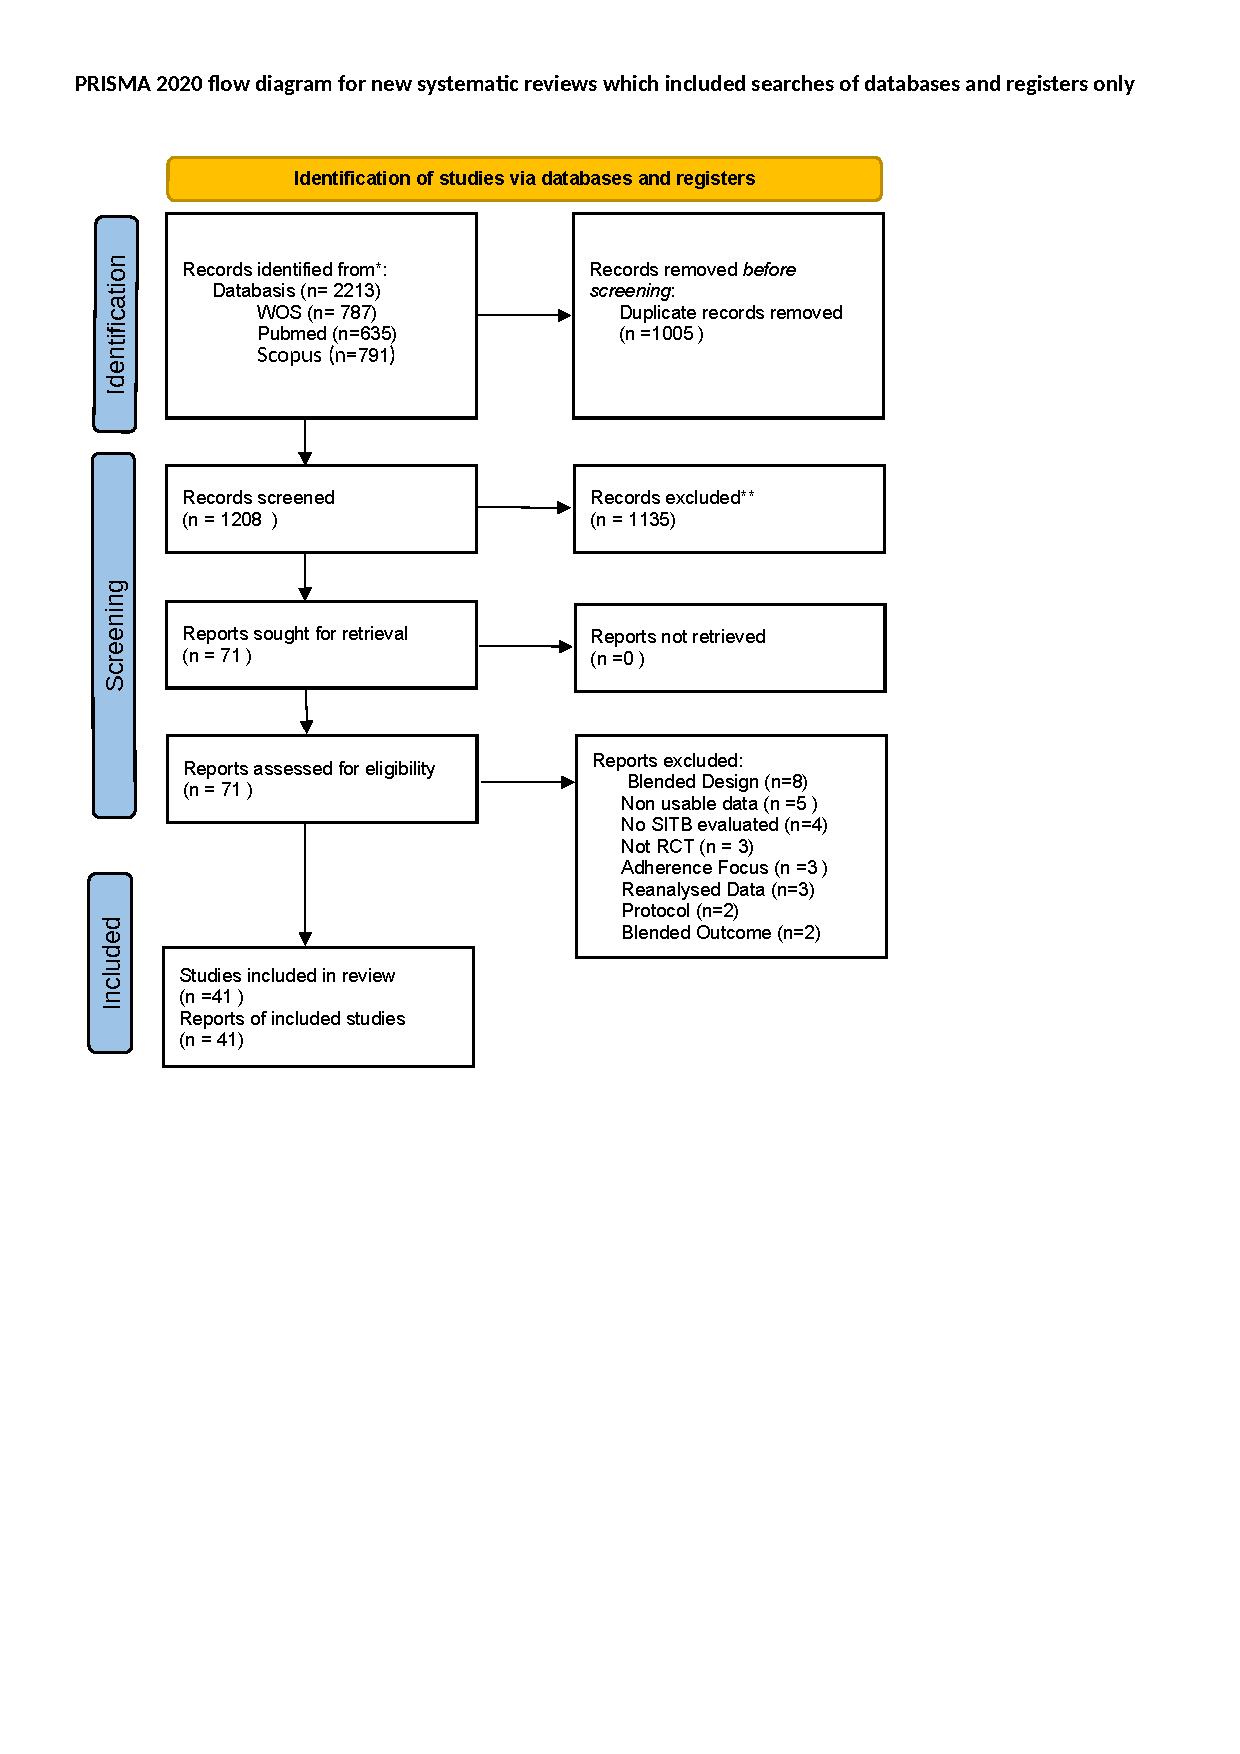
\includegraphics{01_Plots/DBI_Flow_Chart.pdf}
\caption{Flow Chart of all studies}
\end{figure}

Overall, 121 outcomes emerged, with 65 outcomes of the category thinking, predominantly ideation and planning, and 56 outcomes of the category acting, including studies examining mostly deliberate self-harm, self-harm and suicide attempts.

27 outcomes were found in the human involved interventions category and 94 outcomes were found for autonomous interventions. The median duration of studies was 26.00 weeks, with a range of 0.14 to 782 weeks. The median time between post-intervention measures and follow up measures was 17 weeks, with a range of 522 weeks to 0.86 weeks.

The median attrition rate was 30.00 \% with a maximum of 64.50 \% and a minimum of 0 \%.\\

\hypertarget{sample-characteristics}{%
\subsubsection{Sample Characteristics}\label{sample-characteristics}}

The studies included a total of 12821 at post-intervention 9201 at follow up. Out of all, 62.88 \% female and on average 30.80 (SD= 9.95) years old. In studies the youngest reported mean sample age was 14.70 (SD= 1.4) years, the oldest mean sample age was 51.00 (SD= 11.3)years.

Out of a total of n= 37 studies, most data was retrieved from westernised educated industrialised democracies (WEIRD), predominantly the United States (\emph{k=} 10), followed by Australia (\emph{k} = 8). From non-westernised educated industrialised democracies \emph{k = 6} studies emerged.

\hypertarget{main-analysis}{%
\subsection{Main Analysis}\label{main-analysis}}

Distance Based Interventions were effective against suicidal thoughts and behaviours, standardized mean difference (SMD) = -0.11 CI95\%{[}-0.16; -0.07{]}; Heterogeneity was significant at \emph{Q} (df = 114)= 160.42, \emph{p =} 0.00.

Distance based Interventions are more effective against suicidal thoughts than suicidal behaviours (\emph{SMD=} -0.11 CI95\%{[}-0.18; -0.05{]}). The average effectiveness against suicidal thoughts was \emph{SMD=} -0.17 CI95\%{[}-0.24; -0.10{]}, while suicidal behaviours were reduced at around \emph{SMD=} -0.06 CI95\%{[}-0.08; -0.03{]}. Heterogeneity was non-significant \emph{Q} (df = 113) = 124.67, \emph{p =} 0.21. See Appendix C for study average effects against suicidal thoughts and suicidal acts.

Given small study numbers, the comparison of waitlist and attention placebo groups showed statistically not trustworthy results according to the profile likelihood plots.

Therefore, waitlist and attention placebo were combined into a combined control group, and compared to TAU.

Comparing the combined control-group vs.~TAU, retuned that Distance Based Interventions giving alongside TAU were significantly less effected (S\emph{MD=} -0.17 CI95\%{[}-0.26; -0.08{]}), than studies giving Distance Based Interventions using a waitlist or attention placebo control group. Heterogeneity remained significant at \emph{Q} (df = 113) = 146.85, \emph{p =} 0.02.

Covariance was investigated by simultaneous visualization of control-group and outcome category. Suicidal behaviours and suicidal thoughts were unevenly distributed between different control-group types (see figure 2).

An exploratory analysis including both moderators was implemented.

When including both moderators, the difference between control groups became non- significant, with \emph{SMD=} 0.05 CI95\%{[}-0.05; 0.14{]}, but suicidal acts and suicidal thoughts remained a significant moderator, with \emph{SMD =} -0.10 CI95\%{[}-0.18; -0.01{]} in favour of suicidal thoughts; heterogeneity was not significant at \emph{Q} (df = 112) = 124.29, \emph{p =} 0.20.

\begin{figure}
\centering
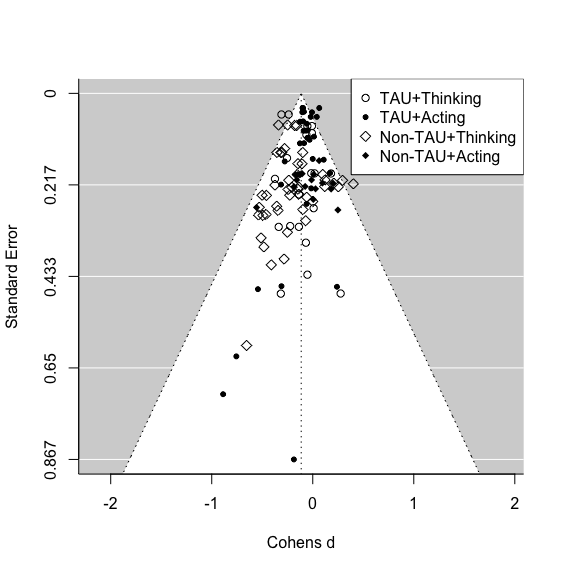
\includegraphics{01_Plots/Rplot2.png}
\caption{Funnel Plot, including all outcomes according to moderator type}
\end{figure}

Effectiveness of Distance Based Interventions decreased between time-points at \emph{SMD =} 0.03 CI95\%{[}-0.02; 0.08{]} non-significantly. Heterogeneity was significant at \emph{Q} (df = 113) = 158.54, \emph{p =} 0.00.

Human involvement had with \emph{SMD=} -0.06 CI95\%{[}-0.14; 0.02{]} an non-significant negative impact on effectiveness. Heterogeneity was significant at \emph{Q} (df = 113) = 153.27, \emph{p =} 0.01.

\hypertarget{sensitivity-analysis-1}{%
\subsection{Sensitivity Analysis}\label{sensitivity-analysis-1}}

Both, inclusion of NSSI (k = 6) and exclusion of suicide studies (k= 4) had negligible impacts on the subgroup of behaviour outcomes. Inclusion of NSSI increased the effectiveness SMD= -0.06 to SMD= -0.09. and exclusion of suicide studies decreased effectiveness from SMD = -0.09 to SMD= -0.05.

\hypertarget{publication-bias-and-risk-of-bias-assessment}{%
\subsection{Publication Bias and Risk of Bias Assessment}\label{publication-bias-and-risk-of-bias-assessment}}

Risk of bias of all \emph{independent} studies was mixed (see Figure 3.). Using Trim and Fill, no publication bias could be observed.

\begin{figure}
\centering
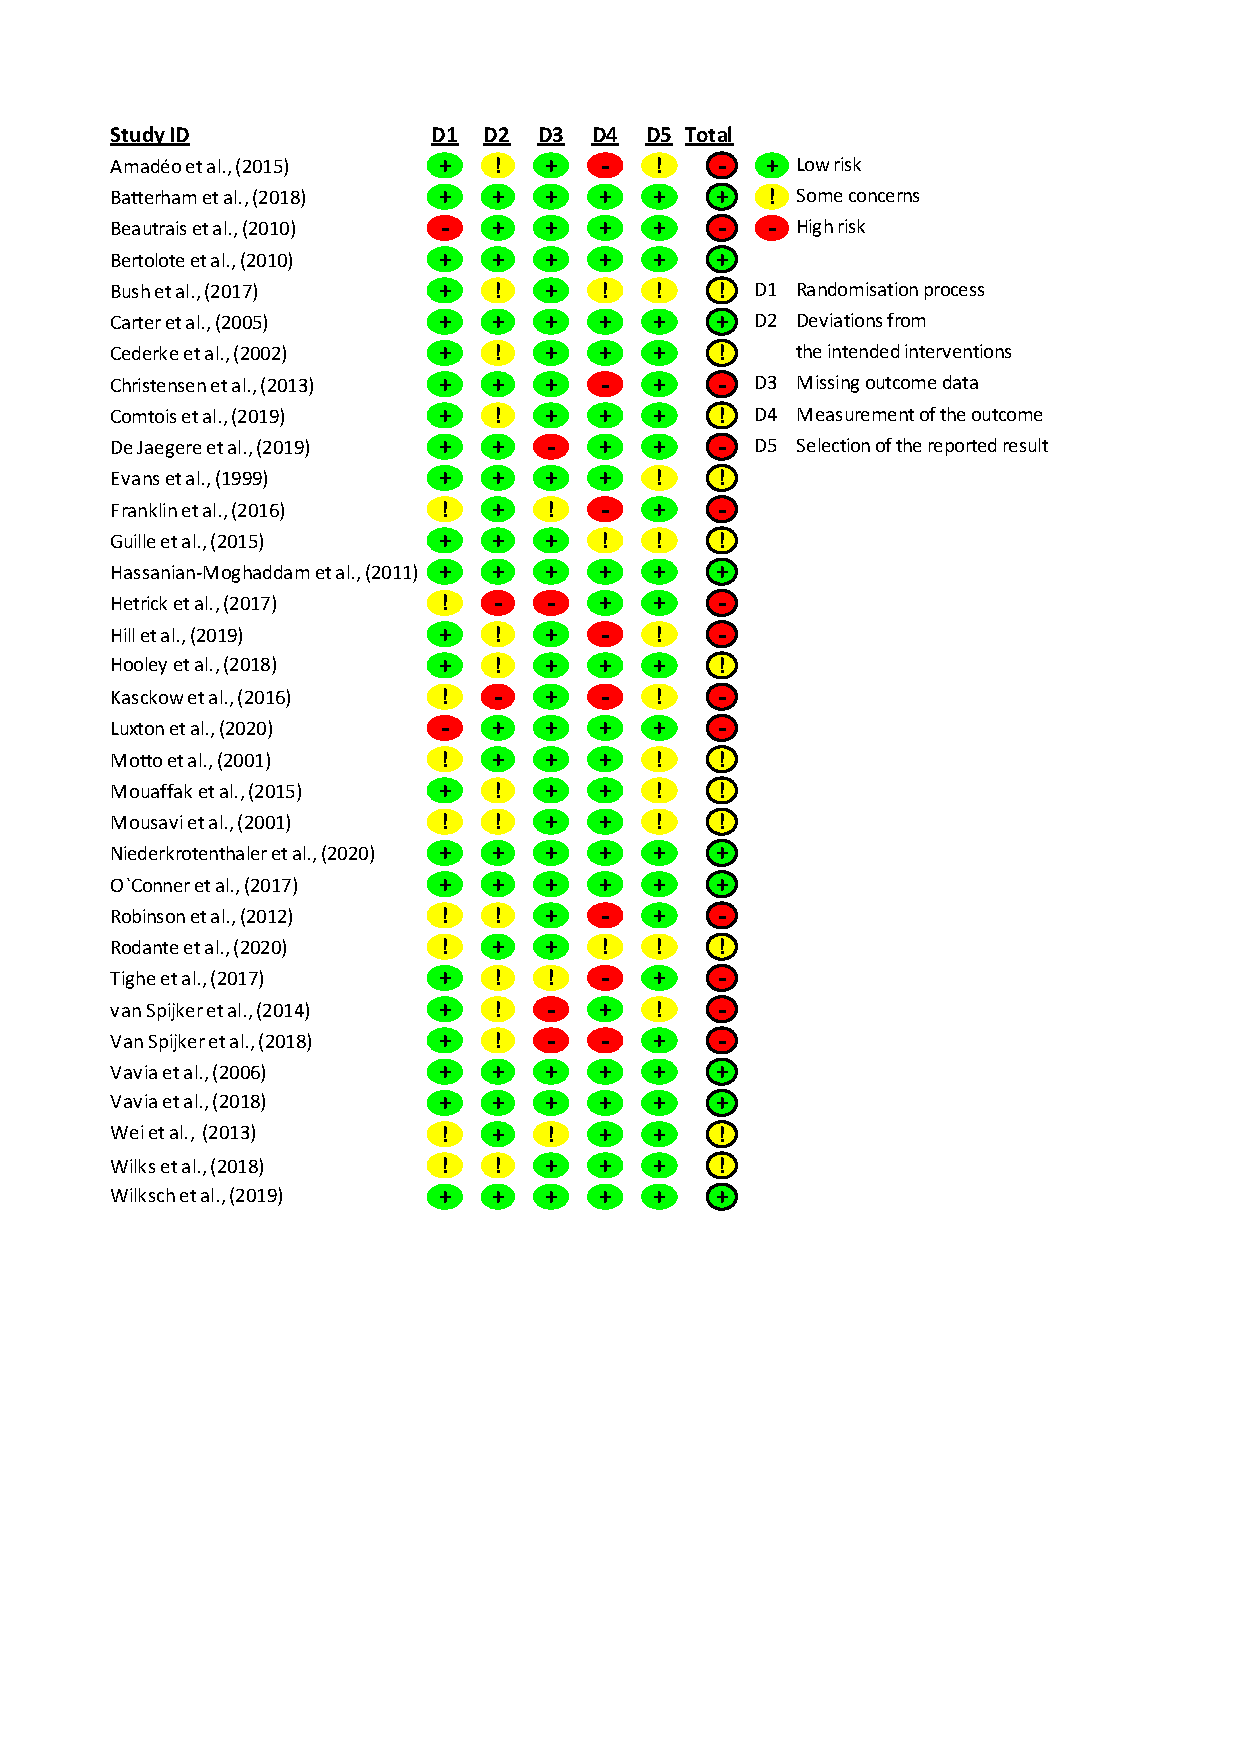
\includegraphics{01_Plots/RoB-II.pdf}
\caption{Quality Assessment of all independent studies}
\end{figure}

\hypertarget{discussion}{%
\section{Discussion}\label{discussion}}

In this meta-analysis we investigated the effectiveness of distance based programs in reducing suicidal thoughts and behaviours. On average distance based programs reduced both suicidal thoughts and behaviours. The quality of evidence was good, given a considerable number of RCTs, with a notable number of high and medium quality studies and no observed publication bias.

\hypertarget{contextualising-results-with-other-meta-analyses}{%
\subsubsection{Contextualising results with other Meta-Analyses}\label{contextualising-results-with-other-meta-analyses}}

To contextualise our results and define where Distance Based Interventions are best used, we searched Web of Science for all meta-analysis published between 2021 and 2018 using ``suic'' and ``therap*.''

\hypertarget{effectiveness-of-distance-based-programs-for-suicidal-behaviours}{%
\paragraph{Effectiveness of distance based programs for suicidal behaviours}\label{effectiveness-of-distance-based-programs-for-suicidal-behaviours}}

We showed that suicidal behaviours were reduced (-0.06 CI95\%{[}-0.08; -0.03{]}) by distance based programs.

Our search returned two meta-analysis that reported on reductions of suicidal behaviours, due to face-to-face interventions, without limiting itself to any specific population (Briggs et al., 2019; Hofstra et al., 2020). While both meta-analysis have their own limitations, Briggs et al. (2019) only including psycho-analytical treatments and Hofstra et al. (2020) including any intervention published between 2011-2017 which includes a control group, these are the closest to general and representative for the research field.

Starting with the therapy unspecific results. Suicide attempts are reduced significantly more effective than Distance Based Interventions by outpatient speciality mental health setting interventions (SMD =-0.705 {[}95\% CI -1.275; -0.135{]}) Hofstra et al. (2020), followed by psychiatric wards in general hospitals (SMD=-0.483{[}95\% CI -0.892; -0.073{]}) and emergency room setting suicide prevention (SMD=-0.319 {[}95\% CI -0.528; -0.110{]}). All of these results have very large confidence intervals, in turn none differ significantly and psychiatric wards in general hospitals do not even differ significantly from Distance Based Interventions in their effectiveness. But, given their mean effect sizes, it is more than reasonable to expect that all these intensive intervention prove superior, given more research.

For therapy specific interventions, namely psychoanalytic face-to-face interventions, Briggs et al. (2019) reported non-significantly stronger results, for suicide attempts \emph{SMD =} -0.24 CI95\%{[}-0.50;0.03{]} and partially significantly stronger results for self harm, ranging between \emph{SMD}= -0.73 CI95\% {[}-1.22;-0.22{]} and \emph{SMD}= -0.15 CI95\% {[}-3.88;0.09{]}; depending on how self harm was measured. The results for suicide attempts where non-significantly different between Briggs et al. (2019) psychoanalytical interventions and any form of intervention of Hofstra et al. (2020). This again shows how underpowered suicide research often is.

Given that only a meta-analysis for psycho-analytical treatments emerged, it maybe argued that other treatments are more effective against suicidal behaviours, such as MBT, DBT, CBT. To argue for or against this point we have to include meta-analysis using youth samples, as no meta-analysis investigating this point emerged for the general population. Drawing on this network meta-analysis (NMA) (Bahji et al., 2021) we can observe strong mostly statistically non-significant difference between different therapy schools. For self harm at the end of therapy the strongest results were delivered by eclectic therapy (ET), followed by dialectical behavioural therapy and short-term psychoanalytic psychotherapy (STPP), the worst results were delivered by brief Interventions, cognitive analytic therapy and family-based therapy (FT). At follow up best were metallization-based therapy, STPP and cognitive behavioural therapy, the worst were FT, supportive therapy, ET. Of note is that the intervention with the best outcome at the end of the treatment ET was the worst at follow up, leading to an increase in self harm (\emph{SMD}= 0.6498{[}CI95\% 0.006; 1.29{]}).

Based on these results, at least in youth and adolescent samples, psycho-analytical approaches are among the most effective forms of therapy to treat self harm. But again research activity is mostly to low to actually differentiate therapies into significantly more and less effective therapies. Although this comparison shows that it is reasonable to treat psychoanalytical therapies as representative for face-to-face interventions for comparison to Distance Based Interventions.

Although distance-based interventions seem to have a small effect size in comparison to face-to face interventions, especially high-frequency long-term interventions and inpatient treatment. We can also see where Distance Based Interventions have a role in the prevention of suicidal behaviour due to their availability, scalability and cost-efficacy.

Even more, it remains to be analysed, whether the higher effectiveness of face-to-face interventions, which is based on rather small samples, would remain superior when their power would be increased. For example, although the effect size of the meta-analysis by Briggs et al. (2019) is likely four times higher than the effect size of Distance Based Interventions, the effect reported here is based on a larger data set, therefore significant, while the likely larger effect sizes in Briggs et al. (2019) remain insignificant, due to low power.

When we also draw on the effect-size estimates and their confidence intervals, we can observe the clinical potential of an intervention. For example, the effect size reported by Briggs et al. (2019) against suicide attempts, expressed as Number Needed to Treat, (NNT) is = 7.4 CI95\% {[}Inf; 3.6{]}, means that the interventions may be ineffective (Infinite number needed), but it could help up to every fourth person. In contrast, our results of distance based programs, expressed as \emph{NNT =} 29.5 CI95\% {[}59; 22.1{]} means that a reduction will occur with 95\% certainty, but \emph{at best} only every twenty-second person will be helped and on average one of 30 interventions will be helpful. Given the seriousness of suicidal behaviours and the currently low effectiveness of interventions against it, more research on potentially more effective treatment is needed. For example, we suggest more research into high frequency interventions and on the question if the trend of larger effect-sizes in psychoanalytical therapies (Briggs et al., 2019) and other promising approaches is retained, given more data. However, despite the low effect of distance based programs on suicidal behaviour, they nevertheless might have a role in the spectrum of preventive approaches. Especially the fact of high barriers to treatment seeking, especially to face-to-face treatment, are an argument to disseminate Distance Based Interventions as a means for involvement where other treatment is not available or not accepted by those in need.

\hypertarget{effectiveness-of-distance-based-programs-for-suicidal-thoughts}{%
\subsubsection{Effectiveness of distance based programs for suicidal thoughts}\label{effectiveness-of-distance-based-programs-for-suicidal-thoughts}}

Similarly to suicidal behaviours, suicidal thoughts were reduced by distance based programs (-0.17 CI95\%{[}-0.24; -0.10{]}).

As the two meta-analysis using general populations (Briggs et al., 2019; Hofstra et al., 2020) did not include any suicidal thoughts measures a direct contextualisation is not possible. Instead we collected all meta-analysis, which used specific populations and reported suicide ideation scores. We assume that if the scores are comparable over different specific populations, they can be generalized.

In total 4 meta-analysis (Bahji et al., 2021; Bornheimer, Zhang, Li, Hiller, \& Tarrier, 2020; Chen, Cheng, Zhao, \& Zhang, 2021; Kothgassner, Robinson, Goreis, Ougrin, \& Plener, 2020) emerged. Of these two (Bahji et al., 2021; Kothgassner, Robinson, Goreis, Ougrin, \& Plener, 2020) used youth samples and two used clinical samples, one of paitents with psychosis (Bornheimer, Zhang, Li, Hiller, \& Tarrier, 2020) and one of patients with BPD (Chen, Cheng, Zhao, \& Zhang, 2021). One meta-analysis used a NMA (Bahji et al., 2021), the rest used Hedges-Olkin approaches.

Reported reductions of suicide ideation did not differ between studies: SMD= -0.17 (95\% CI:-0.33; -0.017) (Bornheimer, Zhang, Li, Hiller, \& Tarrier, 2020), SMD = -0.31, {[}95\% CI: -0.50;--0.12{]} (Kothgassner, Robinson, Goreis, Ougrin, \& Plener, 2020) and SMD = -0.26, {[}95\% CI: -0.74;0.21{]} (Chen, Cheng, Zhao, \& Zhang, 2021); Bahji et al. (2021) NMA did not report a study average effect. Both Bahji et al. (2021) and Kothgassner, Robinson, Goreis, Ougrin, and Plener (2020) reported effects split up according to the psychotherapeutic schools, regarding suicide ideation measures, none differed significantly form one another.

Given the stability of suicide ideation reductions other different populations, psychotherapeutic schools and methods, we see it as possible, to make a cautious comparison between the results of these meta-analysis and the results of our Distance Based Interventions, even though populations differed.

Results of Distance Based Interventions are line with face-to-face interventions according to (Bahji et al., 2021; Bornheimer, Zhang, Li, Hiller, \& Tarrier, 2020; Chen, Cheng, Zhao, \& Zhang, 2021; Kothgassner, Robinson, Goreis, Ougrin, \& Plener, 2020). With only one face-to face interventions significantly exceeded the effectiveness of Distance Based Interventions and only at follow up, not at post treatment, namely mentalization-based therapy (SMD =--1.22 {[}CI95\%: -2.18; --0.26{]} (Bahji et al., 2021).

\hypertarget{research-recommendations}{%
\subsubsection{Research recommendations}\label{research-recommendations}}

According to our results, autonomous distance based interventions (ADBI) (SMD= -0.13 CI95\%{[}-0.19; -0.07{]}), were as effective as human involved interventions (SMD= -0.07 CI95\%{[}-0.12; -0.02{]}). But ADBI promise a better scalability (Batterham et al., 2015), making them more feasible for studies with larger sample sizes and replication studies; something that holds true for almost any psychotherapeutic intervention.

Studies with large sample sizes or study sets using close replications are needed, as only these allow us to control for the characteristics of distance based interventions and by such, to understand which components are most effective.

In general, the assumptions about Distance Based Interventions (DBI) for mental health often lack evidence (Musiat, Goldstone, \& Tarrier, 2014). For example, some stated advantages of Distance Based Interventions in suicide prevention are still unproven assumptions, for example that 24h availability of such an intervention might be advantageous. The best proven assumptions derived from meta-analytical evidence are delivered for cost effectiveness, acceptability and satisfaction of DBIs. However, this evidence is available for mental health interventions in general (Eze, Mateus, \& Cravo Oliveira Hashiguchi, 2020; Musiat, Goldstone, \& Tarrier, 2014), but not for the primary endpoint of suicidal behaviour or thoughts.

In this sense, the development of well powered ADBIs for suicide prevention is still is in its infancy and needs to addressed in future more scrupulously.

\hypertarget{implications-for-clinical-practice}{%
\subsubsection{Implications for clinical practice}\label{implications-for-clinical-practice}}

\hypertarget{placing-distance-based-interventions-on-the-stepped-care-model}{%
\paragraph{Placing Distance Based Interventions on the stepped care model}\label{placing-distance-based-interventions-on-the-stepped-care-model}}

The stepped care model for suicide care (Jobes, Gregorian, \& Colborn, 2018) includes 5 levels of intervention, ranging from least restrictive Telephone (level 1), Brief interventions (2), outpatient care (3), partial hospitalisation (4) to most restrictive interventions like inpatient care/full hospitalisation(5).

As such both the least costly and restrictive level of stepped care, `telephone interventions and follow ups' and the second least costly and restrictive level, `Brief interventions and follow ups' can be supplemented or supplanted by Distance Based Intervention. Further, given that effect-sizes of Distance Based Interventions were similar to other face-to-face interventions, e\underline{ven the remaining three levels can be supplemented by Distance Based Interventions. But should no longer be supplanted by Distance Based Interventions, due to the lack of effectivness against suicidal behaviours and the seriousness of suicide attempts.}

For the best time to intervene this meta-analysis, together with observed meta-analysis shows that all interventions, face-to-face-, Human-Involved Distance Based- as well as autonomous Interventions, at all time-points, are effective in reducing suicide. But, all of these interventions were more effective against suicidal thoughts than against suicidal acts. Therefore, there is a strong argument for the implementation of such interventions among individuals with suicide ideation, as recently discussed by Jobes and Joiner (2019) .

The availability of face-to-face interventions in mental health clinics and among individual mental health professionals such as psychiatrists and psychotherapists is unevenly distributed geographically (Kapusta et al., 2010; Pirkola, Sund, Sailas, \& Wahlbeck, 2009) and may be limited in pandemic containment efforts against Covid-19. The resulting unavailability may be compensated for by ADBIs, which are not affected by geographic distribution or lockdowns. In addition the reality of psychiatric treatment includes high costs for individuals or the public health system (Wittchen et al., 2011), depending on whether psychiatric treatment is covered by insurance. This often results in long waiting times for patients in need (Zepf, Mengele, \& Hartmann, 2003). In both cases, ADBIs can help mitigate the negative effects of barriers to help seeking, by offering an intermediate alternative, thereby bridging waiting times and at lower costs. Finally ADBI can help to scale up mental health services especially in countries with limited mental health expenditures and low resources, such as low and middle income countries (LMIC), as called by Chisholm et al. (2007) and thereby contribute to the Sustainable Mental Health Development Goals, set out be the UN (Patel et al., 2018).

\hypertarget{limitations}{%
\subsection{Limitations}\label{limitations}}

Given our comprehensive approach, some limitations should be noted. Firstly, we did not include any grey literature. This can cause selection bias, as the publication bias suppresses non-significant results. However RCT studies in a multidisciplinary field a rather unlikely. We expect non-publication due to reporting non-significant results is unlikely, given that almost all considered studies included non-significant results. This decision reduced work load notably and is in line with previous meta-analyses to this field (Milner, Carter, Pirkis, Robinson, \& Spittal, 2015 ; Torok et al., 2020).

The second potential limitation is that most studies included in this meta-analysis are already covered by different previously published meta-analyses (Milner, Carter, Pirkis, Robinson, \& Spittal, 2015; Torok et al., 2020). However, these previously published meta-analyses used the Hedges-Olkin meta-analysis which allows only the inclusion of one independent data point, in contrast to our MLM analysis, which allows inclusion of all relevant data (Cheung, 2019).

Utilizing all relevant data has multiple advantages, such as higher precision (a) and less bias risk(b). (a) Including multiple non independent data points per study increases precision. Further it allows important moderator analysis to be implemented in one model, which allows to weigh evidence according to its information value. In contrast, previous meta-analysis had to use independent subgroup analyses, which lowers precision notably and only allows for an indirect comparisons of effectiveness. (b) Bias risk, as stated Hedges-Olkin meta-analyses (Milner, Carter, Pirkis, Robinson, \& Spittal, 2015; Torok et al., 2020) must select one outcome per independent analysis. This can result in a selection bias can be introduced therefore not be excluded in these older meta-analyses. Based on these points and the fact that we updated and broaden the systematic searches of previous meta-analysis, the current meta-analysis substantially adds to the research field.

Despite the above stated advantages a multilevel meta-analysis produces further potential limitations. First, the employed method requires more studies to reach adequate power. The number of included studies was relatively low, thus potentially leading to underpowered results (Tanner-Smith \& Tipton, 2014). But results were reliable, based on Profile Likelihood Plots ( R package \emph{metafor)} and the reported degrees of freedom reported by the RVE Correction (R package \emph{clubsandwich}) (Pustejovsky \& Tipton, 2016). Second, RVE corrected models do not report heterogeneity estimations, therefore heterogeneity estimations of the MLM were reported. However \emph{Q-} test results are not biased by dependency and therefore statistically valid, while power of the \emph{Q}-Test was sufficient (Maeda \& Harwell, 2016).

\hypertarget{conclusion}{%
\subsection{Conclusion}\label{conclusion}}

The presented results of the MLM are based on 37 published peer-reviewed RCT trials on Distance Based Interventions. With an adequate power, no indication for publication bias and manageable heterogeneity. The results suggest that DBI, particularly autonomous Distance Based Interventions, are an effective and affordable possibility to support treatment, specifically against suicidal thoughts and in situations where availability of face-to-face treatments is limited. These results are encouraging as affordable and available DBI mean higher accessibility, in turn promising a reduction of human suffering and health care costs.

\hypertarget{references}{%
\section{References}\label{references}}

\begingroup
\setlength{\parindent}{-0.5in}
\setlength{\leftskip}{0.5in}

References marked with an asterisk indicate studies included in the meta-analysis.

\hypertarget{refs}{}
\begin{CSLReferences}{1}{0}
\leavevmode\hypertarget{ref-amadeo2015}{}%
* Amadeo, S., Rereao, M., Malogne, A., Favro, P., Nguyen, N. L., Jehel, L., \ldots{} De Leo, D. (2015). Testing brief intervention and phone contact among subjects with suicidal behavior: A randomized controlled trial in {French Polynesia} in the frames of the {World Health Organization}/{Suicide Trends} in {At}-{Risk Territories} study. \emph{Mental Illness}, \emph{7}(2), 48--53. \url{https://doi.org/10.4081/mi.2015.5818}

\leavevmode\hypertarget{ref-americanpsychiatricassociation2013a}{}%
American Psychiatric Association. (2013). \emph{Diagnostic and {Statistical Manual} of {Mental Disorders}: Dsm-5}. {Amer Psychiatric Pub Incorporated}. Retrieved from \url{https://books.google.de/books?id=EIbMlwEACAAJ}

\leavevmode\hypertarget{ref-bahji2021}{}%
Bahji, A., Pierce, M., Wong, J., Roberge, J. N., Ortega, I., \& Patten, S. (2021). Comparative {Efficacy} and {Acceptability} of {Psychotherapies} for {Self}-harm and {Suicidal Behavior Among Children} and {Adolescents}: A {Systematic Review} and {Network Meta}-analysis. \emph{JAMA Network Open}, \emph{4}(4), e216614. \url{https://doi.org/10.1001/jamanetworkopen.2021.6614}

\leavevmode\hypertarget{ref-batterham2018}{}%
* Batterham, P. J., Calear, A. L., Farrer, L., McCallum, S. M., \& Cheng, V. W. S. (2018). {FitMindKit} : Randomised controlled trial of an automatically tailored online program for mood, anxiety, substance use and suicidality. \emph{Internet Interventions}, \emph{12}, 91--99. \url{https://doi.org/10.1016/j.invent.2017.08.002}

\leavevmode\hypertarget{ref-batterham2015}{}%
Batterham, P. J., Ftanou, M., Pirkis, J., Brewer, J. L., Mackinnon, A. J., Beautrais, A., \ldots{} Christensen, H. (2015). A systematic review and evaluation of measures for suicidal ideation and behaviors in population-based research. \emph{Psychological Assessment}, \emph{27}(2), 501--512. \url{https://doi.org/10.1037/pas0000053}

\leavevmode\hypertarget{ref-beautrais2010}{}%
* Beautrais, A. L., Gibb, S. J., Faulkner, A., Fergusson, D. M., \& Mulder, R. T. (2010). Postcard intervention for repeat self-harm: Randomised controlled trial. \emph{British Journal of Psychiatry}, \emph{197}(1), 55--60. \url{https://doi.org/10.1192/bjp.bp.109.075754}

\leavevmode\hypertarget{ref-bertolote2010}{}%
* Bertolote, J. M., Fleischmann, A., De Leo, D., Phillips, M. R., Botega, N. J., Vijayakumar, L., \ldots{} Wasserman, D. (2010). Repetition of {Suicide Attempts}: Data from {Emergency Care Settings} in {Five Culturally Different Low}- and {Middle}-{Income Countries Participating} in the {WHO SUPRE}-{MISS Study}. \emph{Crisis-the Journal of Crisis Intervention and Suicide Prevention}, \emph{31}(4), 194--201. \url{https://doi.org/10.1027/0027-5910/a000052}

\leavevmode\hypertarget{ref-borges2010}{}%
Borges, G., Nock, M. K., Haro Abad, J. M., Hwang, I., Sampson, N. A., Alonso, J., \ldots{} Kessler, R. C. (2010). Twelve-{Month Prevalence} of and {Risk Factors} for {Suicide Attempts} in the {World Health Organization World Mental Health Surveys}. \emph{Journal of Clinical Psychiatry}, \emph{71}(12), 1617--1628. \url{https://doi.org/10.4088/JCP.08m04967blu}

\leavevmode\hypertarget{ref-bornheimer2020}{}%
Bornheimer, L. A., Zhang, A., Li, J., Hiller, M., \& Tarrier, N. (2020). Effectiveness of {Suicide}-{Focused Psychosocial Interventions} in {Psychosis}: A {Systematic Review} and {Meta}-{Analysis}. \emph{Psychiatric Services}, \emph{71}(8), 829--838. \url{https://doi.org/10.1176/appi.ps.201900487}

\leavevmode\hypertarget{ref-briggs2019}{}%
Briggs, S., Netuveli, G., Gould, N., Gkaravella, A., Gluckman, N. S., Kangogyere, P., \ldots{} Lindner, R. (2019). The effectiveness of {Psychoanalytic}/{Psychodynamic} psychotherapy for reducing suicide attempts and self-harm: Systematic review and meta-analysis. \emph{The British Journal of Psychiatry : The Journal of Mental Science}, \emph{214}(06), 320--328. \url{https://doi.org/10.1192/bjp.2019.33}

\leavevmode\hypertarget{ref-bruffaerts2011}{}%
Bruffaerts, R., Demyttenaere, K., Hwang, I., Chiu, W.-T., Sampson, N., Kessler, R. C., \ldots{} Nock, M. K. (2011). Treatment of suicidal people around the world. \emph{The British Journal of Psychiatry}, \emph{199}(1), 64--70. \url{https://doi.org/10.1192/bjp.bp.110.084129}

\leavevmode\hypertarget{ref-bush2017}{}%
* Bush, N. E., Smolenski, D. J., Denneson, L. M., Williams, H. B., Thomas, E. K., \& Dobscha, S. K. (2017). A {Virtual Hope Box}: Randomized {Controlled Trial} of a {Smartphone App} for {Emotional Regulation} and {Coping With Distress}. \emph{Psychiatric Services}, \emph{68}(4), 330--336. \url{https://doi.org/10.1176/appi.ps.201600283}

\leavevmode\hypertarget{ref-carter2007}{}%
* Carter, Gregory L., Clover, K., Whyte, I. M., Dawson, A. H., \& D'Este, C. (2007). Postcards from the {EDge}: 24-{Month} outcomes of a randomised controlled trial for hospital-treated self-poisoning. \emph{British Journal of Psychiatry}, \emph{191}, 548--553. \url{https://doi.org/10.1192/bjp.bp.107.038406}

\leavevmode\hypertarget{ref-carter2013}{}%
* Carter, Gregory L., Clover, K., Whyte, I. M., Dawson, A. H., \& D'Este, C. (2013). Postcards from the {EDge}: 5-{Year} outcomes of a randomised controlled trial for hospital-treated self-poisoning. \emph{British Journal of Psychiatry}, \emph{202}(5), 372--380. \url{https://doi.org/10.1192/bjp.bp.112.112664}

\leavevmode\hypertarget{ref-carter2005}{}%
* Carter, Gregory L., Clover, K., Whyte, I. M., Dawson, A. H., \& Este, C. D. (2005). Postcards from the {EDge} project: Randomised controlled trial of an intervention using postcards to reduce repetition of hospital treated deliberate self poisoning. \emph{BMJ (Clinical Research Ed.)}, \emph{331}(7520), 805. \url{https://doi.org/10.1136/bmj.38579.455266.E0}

\leavevmode\hypertarget{ref-cedereke2002}{}%
* Cedereke, M., Monti, K., \& Ojehagen, A. (2002). Telephone contact with patients in the year after a suicide attempt: Does it affect treatment attendance and outcome? A randomised controlled study. \emph{European Psychiatry}, \emph{17}(2), 82--91. \url{https://doi.org/10.1016/S0924-9338(02)00632-6}

\leavevmode\hypertarget{ref-chen2021}{}%
Chen, S., Cheng, Y., Zhao, W., \& Zhang, Y. (2021). Effects of dialectical behaviour therapy on reducing self‐harming behaviours and negative emotions in patients with borderline personality disorder: A meta‐analysis. \emph{Journal of Psychiatric and Mental Health Nursing}, \emph{28}(6), 1128--1139. \url{https://doi.org/10.1111/jpm.12797}

\leavevmode\hypertarget{ref-cheung2019}{}%
Cheung, M. W.-L. (2019). A {Guide} to {Conducting} a {Meta}-{Analysis} with {Non}-{Independent Effect Sizes}. \emph{Neuropsychology Review}, \emph{29}(4), 387--396. \url{https://doi.org/10.1007/s11065-019-09415-6}

\leavevmode\hypertarget{ref-chisholm2007}{}%
Chisholm, D., Flisher, A. J., Lund, C., Patel, V., Saxena, S., Thornicroft, G., \& Tomlinson, M. (2007). Scale up services for mental disorders: A call for action. \emph{Lancet (London, England)}, \emph{370}(9594), 1241--1252. \url{https://doi.org/10.1016/S0140-6736(07)61242-2}

\leavevmode\hypertarget{ref-christensen2013}{}%
* Christensen, H., Farrer, L., Batterham, P. J., Mackinnon, A., Griffiths, K. M., \& Donker, T. (2013). The effect of a web-based depression intervention on suicide ideation: Secondary outcome from a randomised controlled trial in a helpline. \emph{Bmj Open}, \emph{3}(6), e002886. \url{https://doi.org/10.1136/bmjopen-2013-002886}

\leavevmode\hypertarget{ref-comtois2019}{}%
* Comtois, K. A., Kerbrat, A. H., DeCou, C. R., Atkins, D. C., Majeres, J. J., Baker, J. C., \& Ries, R. K. (2019). Effect of {Augmenting Standard Care} for {Military Personnel With Brief Caring Text Messages} for {Suicide Prevention A Randomized Clinical Trial}. \emph{Jama Psychiatry}, \emph{76}(5), 474--483. \url{https://doi.org/10.1001/jamapsychiatry.2018.4530}

\leavevmode\hypertarget{ref-dejaegere2019}{}%
* De Jaegere, E., van Landschoot, R., van Heeringen, K., van Spijker, B. A. J., Kerkhof, A. J. F. M., Mokkenstorm, J. K., \& Portzky, G. (2019). The online treatment of suicidal ideation: A randomised controlled trial of an unguided web-based intervention. \emph{Behaviour Research and Therapy}, \emph{119}, 103406. \url{https://doi.org/10.1016/j.brat.2019.05.003}

\leavevmode\hypertarget{ref-evans1999}{}%
* Evans, M. O., Morgan, H. G., Hayward, A., \& Gunnell, D. J. (1999). Crisis telephone consultation for deliberate self-harm patients: Effects on repetition. \emph{British Journal of Psychiatry}, \emph{175}, 23--27. \url{https://doi.org/10.1192/bjp.175.1.23}

\leavevmode\hypertarget{ref-eze2020}{}%
Eze, N. D., Mateus, C., \& Cravo Oliveira Hashiguchi, T. (2020). Telemedicine in the {OECD}: An umbrella review of clinical and cost-effectiveness, patient experience and implementation. \emph{PLOS ONE}, \emph{15}(8), e0237585. \url{https://doi.org/10.1371/journal.pone.0237585}

\leavevmode\hypertarget{ref-fernandez2021}{}%
Fernandez, E., Woldgabreal, Y., Day, A., Pham, T., Gleich, B., \& Aboujaoude, E. (2021). Live psychotherapy by video versus {In}‐person: A {Meta}‐analysis of efficacy and its relationship to types and targets of treatment. \emph{Clinical Psychology \& Psychotherapy}, cpp.2594. \url{https://doi.org/10.1002/cpp.2594}

\leavevmode\hypertarget{ref-fernandez-castilla2021}{}%
Fernández-Castilla, B., Declercq, L., Jamshidi, L., Beretvas, S. N., Onghena, P., \& Van den Noortgate, W. (2021). Detecting {Selection Bias} in {Meta}-{Analyses} with {Multiple Outcomes}: A {Simulation Study}. \emph{The Journal of Experimental Education}, \emph{89}(1), 125--144. \url{https://doi.org/10.1080/00220973.2019.1582470}

\leavevmode\hypertarget{ref-franklin2016}{}%
* Franklin, J. C., Fox, K. R., Franklin, C. R., Kleiman, E. M., Ribeiro, J. D., Jaroszewski, A. C., \ldots{} Nock, M. K. (2016). A brief mobile app reduces nonsuicidal and suicidal self-injury: Evidence from three randomized controlled trials. \emph{Journal of Consulting and Clinical Psychology}, \emph{84}(6), 544--557. \url{https://doi.org/10.1037/ccp0000093}

\leavevmode\hypertarget{ref-guille2015}{}%
* Guille, C., Zhao, Z., Krystal, J., Nichols, B., Brady, K., \& Sen, S. (2015). Web-{Based Cognitive Behavioral Therapy Intervention} for the {Prevention} of {Suicidal Ideation} in {Medical Interns}: A {Randomized Clinical Trial}. \emph{JAMA Psychiatry}, \emph{72}(12), 1192. \url{https://doi.org/10.1001/jamapsychiatry.2015.1880}

\leavevmode\hypertarget{ref-hassanian-moghaddam2011}{}%
* Hassanian-Moghaddam, H., Sarjami, S., Kolahi, A.-A., \& Carter, G. L. (2011). Postcards in {Persia}: Randomised controlled trial to reduce suicidal behaviours 12 months after hospital-treated self-poisoning. \emph{British Journal of Psychiatry}, \emph{198}(4), 309--316. \url{https://doi.org/10.1192/bjp.bp.109.067199}

\leavevmode\hypertarget{ref-hedges2010}{}%
Hedges, L. V., Tipton, E., \& Johnson, M. C. (2010). Robust variance estimation in meta-regression with dependent effect size estimates. \emph{Research Synthesis Methods}, \emph{1}(1), 39--65. \url{https://doi.org/10.1002/jrsm.5}

\leavevmode\hypertarget{ref-hetrick2017}{}%
* Hetrick, S. E., Yuen, H. P., Bailey, E., Cox, G. R., Templer, K., Rice, S. M., \ldots{} Robinson, J. (2017). Internet-based cognitive behavioural therapy for young people with suicide-related behaviour ({Reframe}-{IT}): A randomised controlled trial. \emph{Evidence-Based Mental Health}, \emph{20}(3), 76--82. \url{https://doi.org/10.1136/eb-2017-102719}

\leavevmode\hypertarget{ref-hill2019}{}%
* Hill, R. M., \& Pettit, J. W. (2019). Pilot randomized controlled trial of {LEAP}: A selective preventive intervention to reduce adolescents' perceived burdensomeness. \emph{JOURNAL OF CLINICAL CHILD AND ADOLESCENT PSYCHOLOGY}, \emph{48}, S45--S56. \url{https://doi.org/10.1080/15374416.2016.1188705}

\leavevmode\hypertarget{ref-hofstra2020}{}%
Hofstra, E., van Nieuwenhuizen, C., Bakker, M., Özgül, D., Elfeddali, I., de Jong, S. J., \& van der Feltz-Cornelis, C. M. (2020). Effectiveness of suicide prevention interventions: A systematic review and meta-analysis. \emph{General Hospital Psychiatry}, \emph{63}, 127--140. \url{https://doi.org/10.1016/j.genhosppsych.2019.04.011}

\leavevmode\hypertarget{ref-hooley2018}{}%
* Hooley, J. M., Fox, K. R., Wang, S. B., \& Kwashie, A. N. D. (2018). Novel online daily diary interventions for nonsuicidal self-injury: A randomized controlled trial. \emph{BMC Psychiatry}, \emph{18}(1). \url{https://doi.org/10.1186/s12888-018-1840-6}

\leavevmode\hypertarget{ref-jobes2018}{}%
Jobes, D. A., Gregorian, M. J., \& Colborn, V. A. (2018). A stepped care approach to clinical suicide prevention. \emph{Psychological Services}, \emph{15}(3), 243--250. \url{https://doi.org/10.1037/ser0000229}

\leavevmode\hypertarget{ref-jobes2019}{}%
Jobes, D. A., \& Joiner, T. E. (2019). Reflections on {Suicidal Ideation}. \emph{Crisis-the Journal of Crisis Intervention and Suicide Prevention}, \emph{40}(4), 227--230. \url{https://doi.org/10.1027/0227-5910/a000615}

\leavevmode\hypertarget{ref-joiner2005}{}%
Joiner, T. (2005). \emph{Why people die by suicide.} {Cambridge, MA, US}: {Harvard University Press}.

\leavevmode\hypertarget{ref-kapusta2010}{}%
Kapusta, N. D., Posch, M., Niederkrotenthaler, T., Fischer-Kern, M., Etzersdorfer, E., \& Sonneck, G. (2010). Availability of {Mental Health Service Providers} and {Suicide Rates} in {Austria}: A {Nationwide Study}, \emph{61}(12), 6.

\leavevmode\hypertarget{ref-kasckow2016}{}%
* Kasckow, J., Zickmund, S., Gurklis, J., Luther, J., Fox, L., Taylor, M., \ldots{} Haas, G. L. (2016). Using telehealth to augment an intensive case monitoring program in veterans with schizophrenia and suicidal ideation: A pilot trial, 14.

\leavevmode\hypertarget{ref-kothgassner2020}{}%
Kothgassner, O. D., Robinson, K., Goreis, A., Ougrin, D., \& Plener, P. L. (2020). Does treatment method matter? A meta-analysis of the past 20 years of research on therapeutic interventions for self-harm and suicidal ideation in adolescents. \emph{Bord Personal Disord Emot Dysregul}, \emph{7}(1), 9. \url{https://doi.org/10.1186/s40479-020-00123-9}

\leavevmode\hypertarget{ref-luxton2020}{}%
* Luxton, D. D., Smolenski, D. J., Reger, M. A., Relova, R. M. V., \& Skopp, N. A. (2020). Caring {E}‐mails for {Military} and {Veteran Suicide Prevention}: A {Randomized Controlled Trial}. \emph{Suicide and Life-Threatening Behavior}, \emph{50}(1), 300--314. \url{https://doi.org/10.1111/sltb.12589}

\leavevmode\hypertarget{ref-maeda2016}{}%
Maeda, Y., \& Harwell, M. R. (2016). Guidelines for {Using} the {Q Test} in {Meta}-{Analysis}, \emph{28}(1), 18.

\leavevmode\hypertarget{ref-milner2015}{}%
Milner, A. J., Carter, G., Pirkis, J., Robinson, J., \& Spittal, M. J. (2015). Letters, green cards, telephone calls and postcards: Systematic and meta-analytic review of brief contact interventions for reducing self-harm, suicide attempts and suicide. \emph{British Journal of Psychiatry}, \emph{206}(3), 184--190. \url{https://doi.org/10.1192/bjp.bp.114.147819}

\leavevmode\hypertarget{ref-moeyaert2017}{}%
Moeyaert, M., Ugille, M., Natasha Beretvas, S., Ferron, J., Bunuan, R., \& Van den Noortgate, W. (2017). Methods for dealing with multiple outcomes in meta-analysis: A comparison between averaging effect sizes, robust variance estimation and multilevel meta-analysis. \emph{Null}, \emph{20}(6), 559--572. \url{https://doi.org/10.1080/13645579.2016.1252189}

\leavevmode\hypertarget{ref-motto2001}{}%
* Motto, J. A., \& Bostrom, A. G. (2001). A {Randomized Controlled Trial} of {Postcrisis Suicide Prevention}. \emph{Psychiatric Services}, \emph{52}(6), 828--833. \url{https://doi.org/10.1176/appi.ps.52.6.828}

\leavevmode\hypertarget{ref-mouaffak2015}{}%
* Mouaffak, F., Marchand, A., Castaigne, E., Arnoux, A., \& Hardy, P. (2015). {OSTA} program: A {French} follow up intervention program for suicide prevention. \emph{Psychiatry Research}, \emph{230}(3), 913--918. \url{https://doi.org/10.1016/j.psychres.2015.11.024}

\leavevmode\hypertarget{ref-mousavi2014}{}%
* Mousavi, S. G., Zohreh, R., Maracy, M. R., Ebrahimi, A., \& Sharbafchi, M. R. (2014). The efficacy of telephonic follow up in prevention of suicidal reattempt in patients with suicide attempt history. \emph{Advanced Biomedical Research}, 6.

\leavevmode\hypertarget{ref-musiat2014}{}%
Musiat, P., Goldstone, P., \& Tarrier, N. (2014). Understanding the acceptability of e-mental health - attitudes and expectations towards computerised self-help treatments for mental health problems. \emph{BMC Psychiatry}, \emph{14}(1), 109. \url{https://doi.org/10.1186/1471-244X-14-109}

\leavevmode\hypertarget{ref-niederkrotenthaler2020}{}%
* Niederkrotenthaler, T., \& Till, B. (2020). Effects of suicide awareness materials on individuals with recent suicidal ideation or attempt: Online randomised controlled trial. \emph{British Journal of Psychiatry}, \emph{217}(6), 693--700. \url{https://doi.org/10.1192/bjp.2019.259}

\leavevmode\hypertarget{ref-oconnor2017}{}%
* O'Connor, R. C., Ferguson, E., Scott, F., Smyth, R., McDaid, D., Park, A.-L., \ldots{} Armitage, C. J. (2017). A brief psychological intervention to reduce repetition of self-harm in patients admitted to hospital following a suicide attempt: A randomised controlled trial. \emph{The Lancet. Psychiatry}, \emph{4}(6), 451--460. \url{https://doi.org/10.1016/S2215-0366(17)30129-3}

\leavevmode\hypertarget{ref-page2021}{}%
Page, M. J., McKenzie, J. E., Bossuyt, P. M., Boutron, I., Hoffmann, T. C., Mulrow, C. D., \ldots{} Moher, D. (2021). The {PRISMA} 2020 statement: An updated guideline for reporting systematic reviews. \emph{BMJ (Clinical Research Ed.)}, n71. \url{https://doi.org/10.1136/bmj.n71}

\leavevmode\hypertarget{ref-park2019}{}%
Park, S., \& Beretvas, S. N. (2019). Synthesizing effects for multiple outcomes per study using robust variance estimation versus the three-level model. \emph{Behav Res}, \emph{51}(1), 152--171. \url{https://doi.org/10.3758/s13428-018-1156-y}

\leavevmode\hypertarget{ref-patel2018}{}%
Patel, V., Saxena, S., Lund, C., Thornicroft, G., Baingana, F., Bolton, P., \ldots{} UnÜtzer, Jü. (2018). The {Lancet Commission} on global mental health and sustainable development. \emph{The Lancet}, \emph{392}(10157), 1553--1598. \url{https://doi.org/10.1016/S0140-6736(18)31612-X}

\leavevmode\hypertarget{ref-pirkola2009}{}%
Pirkola, S., Sund, R., Sailas, E., \& Wahlbeck, K. (2009). Community mental-health services and suicide rate in {Finland}: A nationwide small-area analysis. \emph{The Lancet}, \emph{373}(9658), 147--153. \url{https://doi.org/10.1016/S0140-6736(08)61848-6}

\leavevmode\hypertarget{ref-pustejovsky2021a}{}%
Pustejovsky, J. E. (2021). \emph{{clubSandwich}: Cluster-robust (sandwich) variance estimators with small-sample corrections}. manual. Retrieved from \url{https://CRAN.R-project.org/package=clubSandwich}

\leavevmode\hypertarget{ref-pustejovsky2016}{}%
Pustejovsky, J. E., \& Tipton, E. (2016). Small sample methods for cluster-robust variance estimation and hypothesis testing in fixed effects models. Retrieved from \url{http://arxiv.org/abs/1601.01981}

\leavevmode\hypertarget{ref-pustejovsky2021}{}%
Pustejovsky, J. E., \& Tipton, E. (2021). Meta-analysis with {Robust Variance Estimation}: Expanding the {Range} of {Working Models}. \emph{Prevention Science}. \url{https://doi.org/10.1007/s11121-021-01246-3}

\leavevmode\hypertarget{ref-rcoreteam2020}{}%
R Core Team. (2020). \emph{R: A language and environment for statistical computing}. manual, {Vienna, Austria}. Retrieved from \url{https://www.R-project.org/}

\leavevmode\hypertarget{ref-renkewitz2019}{}%
Renkewitz, F., \& Keiner, M. (2019). How to {Detect Publication Bias} in {Psychological Research}: A {Comparative Evaluation} of {Six Statistical Methods}. \emph{Zeitschrift für Psychologie}, \emph{227}(4), 261--279. \url{https://doi.org/10.1027/2151-2604/a000386}

\leavevmode\hypertarget{ref-robinson2012}{}%
* Robinson, J., Yuen, H. P., Gook, S., Hughes, A., Cosgrave, E., Killackey, E., \ldots{} Yung, A. (2012). Can receipt of a regular postcard reduce suicide-related behaviour in young help seekers? A randomized controlled trial: A postcard study for at-{Risk} young help seekers. \emph{Early Intervention in Psychiatry}, \emph{6}(2), 145--152. \url{https://doi.org/10.1111/j.1751-7893.2011.00334.x}

\leavevmode\hypertarget{ref-rodante2020}{}%
* Rodante, D. E., Kaplan, M. I., Olivera Fedi, R., Gagliesi, P., Pascali, A., José Quintero, P. S., \ldots{} Daray, F. M. (2020). {CALMA}, a {Mobile Health Application}, as an {Accessory} to {Therapy} for {Reduction} of {Suicidal} and {Non}-{Suicidal Self}-{Injured Behaviors}: A {Pilot Cluster Randomized Controlled Trial}. \emph{Null}, 1--18. \url{https://doi.org/10.1080/13811118.2020.1834476}

\leavevmode\hypertarget{ref-sterne2019}{}%
Sterne, J. A. C., Savović, J., Page, M. J., Elbers, R. G., Blencowe, N. S., Boutron, I., \ldots{} Higgins, J. P. T. (2019). {RoB} 2: A revised tool for assessing risk of bias in randomised trials. \emph{BMJ (Clinical Research Ed.)}, l4898. \url{https://doi.org/10.1136/bmj.l4898}

\leavevmode\hypertarget{ref-tanner-smith2014}{}%
Tanner-Smith, E. E., \& Tipton, E. (2014). Robust variance estimation with dependent effect sizes: Practical considerations including a software tutorial in {Stata} and {\textsc{Spss}}: Robust variance estimation, \emph{5}(1), 13--30. \url{https://doi.org/10.1002/jrsm.1091}

\leavevmode\hypertarget{ref-tighe2017}{}%
* Tighe, J., Shand, F., Ridani, R., Mackinnon, A., De La Mata, N., \& Christensen, H. (2017). Ibobbly mobile health intervention for suicide prevention in {Australian Indigenous} youth: A pilot randomised controlled trial. \emph{BMJ Open}, \emph{7}(1), e013518. \url{https://doi.org/10.1136/bmjopen-2016-013518}

\leavevmode\hypertarget{ref-torok2020}{}%
Torok, M., Han, J., Baker, S., Werner-Seidler, A., Wong, I., Larsen, M. E., \& Christensen, H. (2020). Suicide prevention using self-guided digital interventions: A systematic review and meta-analysis of randomised controlled trials. \emph{The Lancet Digital Health}, \emph{2}(1), e25--e36. \url{https://doi.org/10.1016/S2589-7500(19)30199-2}

\leavevmode\hypertarget{ref-vaiva2018}{}%
* Vaiva, G., Berrouiguet, S., Walter, M., Courtet, P., Ducrocq, F., Jardon, V., \ldots{} Goldstein, P. (2018). Combining {Postcards}, {Crisis Cards}, and {Telephone Contact Into} a {Decision}-{Making Algorithm} to {Reduce Suicide Reattempt}: A {Randomized Clinical Trial} of a {Personalized Brief Contact Intervention}. \emph{The Journal of Clinical Psychiatry}, \emph{79}(6). \url{https://doi.org/10.4088/JCP.17m11631}

\leavevmode\hypertarget{ref-vaiva2006}{}%
* Vaiva, G., Vaiva, G., Ducrocq, F., Meyer, P., Mathieu, D., Philippe, A., \ldots{} Goudemand, M. (2006). Effect of telephone contact on further suicide attempts in patients discharged from an emergency department: Randomised controlled study. \emph{BMJ (Clinical Research Ed.)}, \emph{332}(7552), 1241--1245. \url{https://doi.org/10.1136/bmj.332.7552.1241}

\leavevmode\hypertarget{ref-vandennoortgate2013}{}%
Van den Noortgate, W., López-López, J. A., Marín-Martínez, F., \& Sánchez-Meca, J. (2013). Three-level meta-analysis of dependent effect sizes. \emph{Behavior Research Methods}, \emph{45}(2), 576--594. \url{https://doi.org/10.3758/s13428-012-0261-6}

\leavevmode\hypertarget{ref-vandennoortgate2015}{}%
Van den Noortgate, W., López-López, J. A., Marín-Martínez, F., \& Sánchez-Meca, J. (2015). Meta-analysis of multiple outcomes: A multilevel approach. \emph{Behavior Research Methods}, \emph{47}(4), 1274--1294. \url{https://doi.org/10.3758/s13428-014-0527-2}

\leavevmode\hypertarget{ref-vanspijker2014}{}%
* van Spijker, B. A. J., van Straten, A., \& Kerkhof, A. J. F. M. (2014). Effectiveness of {Online Self}-{Help} for {Suicidal Thoughts}: Results of a {Randomised Controlled Trial}. \emph{PLoS ONE}, \emph{9}(2), e90118. \url{https://doi.org/10.1371/journal.pone.0090118}

\leavevmode\hypertarget{ref-vanspijker2018}{}%
* van Spijker, B. A., Werner-Seidler, A., Batterham, P. J., Mackinnon, A., Calear, A. L., Gosling, J. A., \ldots{} Christensen, H. (2018). Effectiveness of a {Web}-{Based Self}-{Help Program} for {Suicidal Thinking} in an {Australian Community Sample}: Randomized {Controlled Trial}. \emph{Journal of Medical Internet Research}, \emph{20}(2), e15. \url{https://doi.org/10.2196/jmir.8595}

\leavevmode\hypertarget{ref-viechtbauer2010c}{}%
Viechtbauer, W. (2010). Conducting {Meta}-{Analyses} in {R} with the metafor {Package}. \emph{Journal of Statistical Software}, \emph{36}(3). \url{https://doi.org/10.18637/jss.v036.i03}

\leavevmode\hypertarget{ref-wei2013}{}%
* Wei, S., Liu, L., Bi, B., Li, H., Hou, J., Tan, S., \ldots{} Liu, Y. (2013). An {Intervention} and {Follow}-{Up Study Following} a {Suicide Attempt} in the {Emergency Departments} of {Four General Hospitals} in {Shenyang}, {China}. \emph{Crisis-the Journal of Crisis Intervention and Suicide Prevention}, \emph{34}(2), 107--115. \url{https://doi.org/10.1027/0227-5910/a000181}

\leavevmode\hypertarget{ref-wilks2018}{}%
* Wilks, C. R., Lungu, A., Ang, S. Y., Matsumiya, B., Yin, Q., \& Linehan, M. M. (2018). A randomized controlled trial of an {Internet} delivered dialectical behavior therapy skills training for suicidal and heavy episodic drinkers. \emph{Journal of Affective Disorders}, \emph{232}, 219--228. \url{https://doi.org/10.1016/j.jad.2018.02.053}

\leavevmode\hypertarget{ref-wittchen2011a}{}%
Wittchen, H. U., Jacobi, F., Rehm, J., Gustavsson, A., Svensson, M., Jönsson, B., \ldots{} Steinhausen, H.-C. (2011). The size and burden of mental disorders and other disorders of the brain in {Europe} 2010. \emph{European Neuropsychopharmacology}, \emph{21}(9), 655--679. \url{https://doi.org/10.1016/j.euroneuro.2011.07.018}

\leavevmode\hypertarget{ref-worldhealthorganization2021}{}%
World Health Organization. (2021). \emph{Suicide worldwide in 2019: Global health estimates}. {Geneva}: {World Health Organization}. Retrieved from \url{https://apps.who.int/iris/handle/10665/341728}

\leavevmode\hypertarget{ref-zepf2003}{}%
Zepf, S., Mengele, U., \& Hartmann, S. (2003). Zum Stand der ambulanten psychotherapeutischen Versorgung der Erwachsenen in der Bundesrepublik Deutschland. \emph{Psychotherapie, Psychosomatik, medizinische Psychologie}, \emph{53}(3/4), 152--162. \url{https://doi.org/10.1055/s-2003-38004}

\leavevmode\hypertarget{ref-zuromski2019}{}%
Zuromski, K. L., Bernecker, S. L., Gutierrez, P. M., Joiner, T. E., King, A. J., Liu, H., \ldots{} Kessler, R. C. (2019). Assessment of a {Risk Index} for {Suicide Attempts Among US Army Soldiers With Suicide Ideation}: Analysis of {Data From} the {Army Study} to {Assess Risk} and {Resilience} in {Servicemembers} ({Army STARRS}). \emph{JAMA Network Open}, \emph{2}(3), e190766. \url{https://doi.org/10.1001/jamanetworkopen.2019.0766}

\end{CSLReferences}

\endgroup

\hypertarget{appendix}{%
\section{Appendix}\label{appendix}}

\hypertarget{online-supplement-1}{%
\subsection{Online Supplement 1}\label{online-supplement-1}}

\hypertarget{search-strings}{%
\subsubsection{Search Strings:}\label{search-strings}}

Note: Search string was adapted in Scopus adding: TITLE-ABS-KEY. This is implied when using WOS and Pubmed. As in WOS and Pubmed Title, Abstract and Keywords were also searched, both strings are in practice identical.

\hypertarget{for-wos-and-pubmed}{%
\paragraph{For WOS and Pubmed}\label{for-wos-and-pubmed}}

((``Suic*'' OR ``Suicide prevention'' OR ``self harm*'' OR ``self poisoning*'' OR ``self injur*'' OR ``self mutilation'' ) AND (``telehealth''OR``postcard*''OR ``onlin*''OR``Online Intervention'' OR ``Online Prevent*'' OR ``E Intervention'' OR ``E-Intervention'' OR ``E Prevention'' OR ``Electronic Intervention'' OR ``Electronic Prevention'' OR ``Mobile Intervention'' OR ``Mobile Prevention'' OR ``Web-Based*'' OR ``Web Based*''~ OR ``Online Support'' OR ``E Therapy'' OR ``e-mail*'' OR ``e mail*'' OR ``App'' OR ``Apps'' OR ``App-Assis*'' OR ``mobile-App'' OR ``mobile health intervention'' OR ``telephone'' OR ``phone based'' OR ``letter*'') AND (RCT OR Random*))

\hypertarget{scopus}{%
\paragraph{Scopus:}\label{scopus}}

( TITLE-ABS-KEY ( ( ``Suic*''~ OR~ ``Suicide prevention''~ OR~ ``self harm*''~ OR~ ``self poisoning*''~ OR~ ``self injur*''~ OR~ ``self mutilation'' )~ AND~ ( ``telehealth''~ OR~ ``postcard*''~ OR~ ``onlin*''~ OR~ ``Online Intervention''~ OR~ ``Online Prevent*''~ OR~ ``E Intervention''~ OR~ ``E-Intervention''~ OR~ ``E Prevention''~ OR~ ``Electronic Intervention''~ OR~ ``Electronic Prevention''~ OR~ ``Mobile Intervention''~ OR~ ``Mobile Prevention''~ OR~ ``Web-Based*''~ OR~ ``Web Based*''~ OR~ ``Online Support''~ OR~ ``E Therapy''~ OR~ ``e-mail*''~ OR~ ``e mail*''~ OR~ ``App''~ OR~ ``Apps''~ OR~ ``App-Assis*''~ OR~ ``mobile-App''~ OR~ ``mobile health intervention''~ OR~ ``telephone''~ OR~ ``phone based''~ OR~ ``letter*'' )~ AND~ ( rct~ OR~ random* ) ) )


\end{document}
